\chapter{Methods}

The eartgEngineGrabR package is supposed to provide an interface of R and the GEE to acquire remote sensing data in R. The emphasis is to develop a stable framework for an interface between R and the GEE. This framework should enable the user to select from some data sets, choose a temporal and spatial resolution and send a request to the earth engine servers to process and export the data to the user's local machine. The framework is supposed to work as a foundation that eases further extensions.

The base functionality of the framework is: 
\begin{itemize}
	\item uploading vector data to earth engine
	\item select a data product
	\item provide extensive control over the aggregation corresponding to the shape, temporal and spatial resolution
	\item export data products from earth engine and import the products into R
	\item manage the dependencies and authorisations to the involved API's
\end{itemize}

The package consists of two functions \texttt{ee\_grab} and \texttt{ee\_grab\_init}. The \texttt{ee\_grab\_init} function handles authentications and the installation of additional dependencies necessary for the eartgEngineGrabR package to work. The \texttt{ee\_grab} function controlls the acquisition of the remote sensing data from the GEE.

First, the data section gives an overview of the data temporarily accessible through the eartgEngineGrabR package. 
The next section introduces the general design and functionality that the package provides during the acquisition process. The section covers how the \texttt{ee\_grab} function can select, filter, aggregate and retrieve the requested data, while the emphasis lies on the design workflow and arguments of the function.
The following section introduces the technical framework that enables the interface of R and the GEE, while the focus in on the technical side in \texttt{ee\_grab} function call.
The last section covers the necessary dependencies and authentications processes handled by the \texttt{ee\_grab\_init}.

The emphasis of the current version of the earthEngineGraR package and the present thesis is to develop a stable interface of R and the GEE to retrieve data in a user-specific form. Therefore the temporally available data is still limited to a selected list of data products, that should illustrate the diversity of the Earth Engine data catalogue. In the further development of the earthEngineGrabR package, this list should be extended.

\begin{table}[h]
	\begin{tabularx}{\textwidth}{llccc}
		\toprule
		\textbf{data source} & \textbf{data product} & \textbf{spatial} & \textbf{temporal} & \textbf{coverage}\\
		\toprule
		
		MOD44B.051 & tree-cover  & 30 m & yearly & 2000–2015 \\
		
		& non-tree-cover  & 30 m & yearly & 2000–2015 \\
		
		& non-vegetation  & 30 m & yearly & 2000–2015 \\
		
		JRC Global \\ Surface Water  & Distance to surface water & 30 m & yearly & 1984–2015 \\
		
		CHIRPS & precipitation & 0.05$^\circ$ & monthly & 2000–2015\\
		
		SRTM & elevation  & 30 m & Single & 2000\\
		& slope  & 30 m & Single & 2000\\
		
		Oxford MAP & Accessibility to Cities  & 0.01$^\circ$ & Single & 2015\\
		
		& Friction Surface  & 0.01$^\circ$  & Single & 2015\\
		
		\hline
	\end{tabularx}
	\caption{Data products with temporal coverage, temporal-resolution and spatial-resolution available in the earthEngineGraR}
\end{table}

Table A shows the list of data products temporally accessible through the package. In the following, it is distinguished between a data source of the remote sensing data, that represents the primary source, for example, the Modis MOD44B.051 Terra Vegetation Continous Fields (VCF) and the derived data product: percent tree cover. In the earthEngineGrabR, the user requests remote sensing data as specific data products. A data product always represents one band of the source satellite image and one environmental variable like percent-tree-cover, distance-to-surface-water or slope.
The variables vary in temporal and spatial resolution dependent on the data product they are derived from. 

To access land cover, the MOD44B.051 Terra VCF product with a yearly temporal resolution and a 250m spatial resolution is used. The data set provides a sub-pixel-level representation of surface vegetation cover, designed to continuously represent Earth's terrestrial surface as a gradient of three essential surface cover components: percent tree cover, percent non-tree cover and percent bare. The data set is generated using monthly composites of Terra MODIS 250 and 500 meters Land Surface Reflectance data (\cite{hansen2006vegetation}).
The Joint Research Center (JRC), Water Classification History, is a data set, produced in collaboration with the European Commission and Google. The data set provides a pixel-wise classification of surface water generated using, 3,066,102 scenes from Landsat 5, 7 and 8 acquired between 1984 and 2015. Each pixel was individually classified into water and non-water. The data comes in an original monthly temporal resolution and an aggregated yearly resolution (\cite{pekel2016high}). In the earthEngineGrabR, the aggregated yearly water classification data is used, providing a pixel-wise classification of seasonal water, permanent water and not water. To convert this information in an ecological context, the data is further processed to receive the distance to surface water product for each pixel. To compute the distance permanent and seasonal water are merged. Therefore the distance refers to permanent and seasonal water.

To provide topographic products, the Shuttle Radar Topography Mission (SRTM) of NASA acquired in 2007 with a spatial resolution of 30 meters, is used. While the SRTM dataset provides elevation in meters, the slope product is additionally processed in earth engine (\cite{farr2007shuttle}). To account for Socio-economic variables the recently published Oxford MAP datasets of Accessibility to Cities for 2015 and Global Friction Surface for 2015 both with a spatial resolution of $0.01$ ($~ 30m$) are used. The global Friction Surface map estimates land-based travel speed for land pixels in the year 2015, and the global Accessibility map estimates land-based travel time to the nearest densely-populated area for the year 2015 (\cite{weiss2018global}). Both datasets were produced through a collaboration between the Univerity of Oxford Malaria Atlas Project (MAP), Google, the European Union JRC. To produce the maps, the first time a global-scale combination of Open Street Map data and Google roads dataset was used, extended with datasets for topographic conditions, land cover types and national borders.
For the Friction Surface map, these underlying datasets were used to calculate travel speed regarding time to cross each pixel, with the fastest travel mode intersecting the pixel being used to determine the speed to travel in that pixel. The travel speed is in minutes required to travel one meter. The Accessibility map is produced by using the Friction Surface map in combination with a least-cost-algorithm, which calculates the travel time in minutes for each pixel to the nearest city. Cities were determined by using data from the Global Human Settlement Project.  

The Climate Hazard Group InfraRed Precipitation with Station Data (CHIRPS) is a global rainfall data set with a daily temporal resolution and 0.05 spatial resolution (~150m). In the earthEngineGraR package, the CHIRPS daily (version 2.0 final) is utilised, an aggregated version of the daily CHIRPS dataset, with a temporal resolution of 1 days (\cite{funk2015climate}).

For consistency, the data products that have a high spatial resolution like CHIRPS and JRC are only available between 2000 and 2015. This way, there is one corresponding period most data is available in.




\section{How the data is controlled}



Instead of downloading the raw raster data the package provides control to filter and aggregate selected data products according to a given target. This processing allows retrieving the environmental variables in a specific, user-defined format. The user specifies a data product,  a time interval, a temporal reducer, a spatial reducer and a target. In the GEE a reducer is a way to aggregate data over space and time. In the GEE2R package, there are implementations for simple statistics like mean, mode, max, and min. The temporal reducer aggregates the data over time and the spatial reducer aggregates the data over a region defines by the target. 
The target is defined by a shapefile, where the spatial extent of the features define the region the spatial reducer is applied over.

\begin{center}
	\begin{figure}[h]
		\begin{center}
			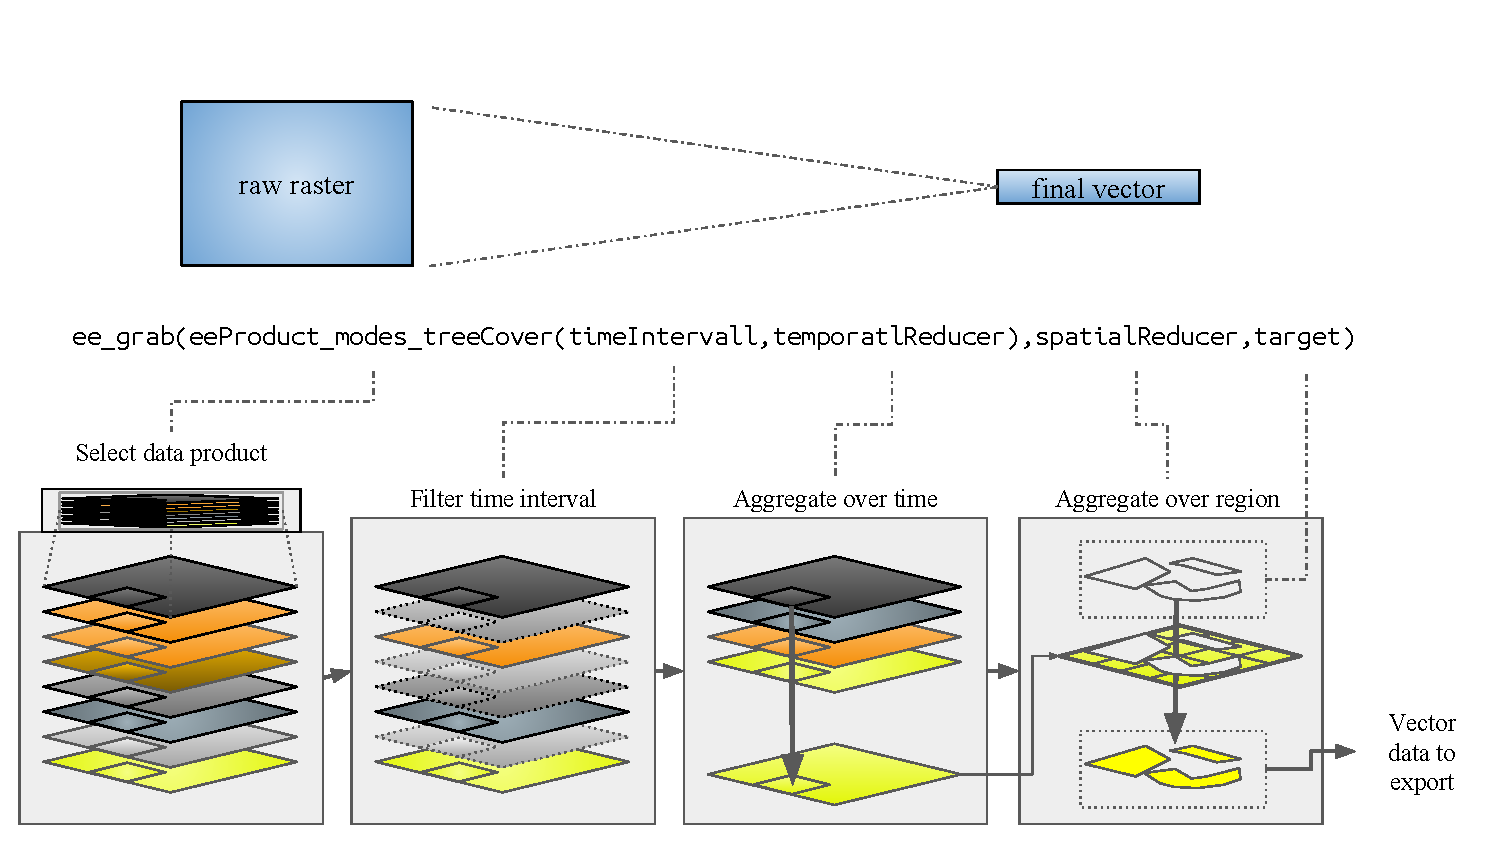
\includegraphics[width=15cm]{images/design_function.pdf}
		\end{center}
	\end{figure}
	% \vskip 2em%
\end{center}

Image 1 shows the basic processing flow to retrieve an environmental variable in a defined format. First, the data product is selected, if the data has a temporal resolution, the time interval is used to filter the data. The images passing the filter are reduced to one image with the given temporal reducer. Next, for each region of the raster overlapping with a feature in the target shapefile a reducer is applied and a statistic is computed. The output of this process is a feature collection in the vector format. This feature collection is exported to the user's local machine.
During this entire processing flow, the size of the data is massively reduced. All 



\section{technical structure}

To enable R users to request and download data from the GEE, the package combines multiple tools like the programming languages R, Python, as well as multiple web services provided by Google like the Fusion Tables, Google Drive and of course the GEE. While Google Drive is a general file sharing and storage service for all kinds of files, Google Fusion Table is specifically designed to manage tabular data and enables to upload, manipulate, visualize and share small amounts of data online.

Each tool performs a specific task. In R, the user specifies the requested data and initializes all further processes. In Python, the actual request is generated and send to the GEE. Because the GEE can import Fusion Tables, the Google Fusion Table is used to upload local vector data to the GEE. The GEE performs all data processing and exports the data to Google Drive wherefrom it's downloaded and imported into R. 


\begin{center}
	
	\begin{figure}[h]
		\begin{center}
			\includegraphics[width=15cm]{images/processin_folw.pdf}
		\end{center}
	\end{figure}
	% \vskip 2em%
\end{center}

Flowchart A shows a schematic sequence of processes that are executed in the main \texttt{ee\_grab} function call. The Flowchart is divided between processes that are performed locally and processes performed by some kind of web server on the cloud. On the local machine, the black box illustrates the function call in the R console while the 3 main folders correspond to the GEE2R library folder, the temporal working directory and the folder for the earth engine python client library. The folders contain two different sorts of files, either the bright R or Python scripts, that execute specific tasks or the dark data files that stands for intermediate products in the processing chain.
At the beginning of the function call, the target vector data is uploaded as Fusion Table illustrated with the dark yellow arrows with number 1. 
The group of processes with the number 2 in red, describes the integration of R and Python and the way python code is executed from R. The processes with number 3 in yellow, represents the exchange of arguments, or,  how parameters are passed from R to Python. The orange arrows with the number 4 illustrate the structure of the python code as executable modules. The blue processes with the number 5 show the communication of the python client library and the GEE while the dark blue arrows with number 6 describe the approach to send process info from GEE to R. In dark grey with number 7 the import of the Fusion Table the computation and the export of the processed data is illustrated and finally the green processes with number 8, describes the access from R to Google Drive and the following download and import of the final data into R.
Based on the classification of the flowchart, the following section explains all 8 groups of processes in detail.

If installed, the GEE2R R library is located in a default library folder for all R libraries. In the GEE2R folder, there is R folder, containing an R script, which defines all R functions used in the package. Furthermore, there is an additional Python folder containing python scripts divided into execution scripts and function scripts. The function script, again, defines all python functions. The execution script, however, is executed from R and uses these functions.

To upload the target vector data the Fusion Table driver in the Geospatial Data Abstraction (GDAL) library is used. To execute GDAL from R, R's ability to invoke function calls is applied, this method will be explained in more detail in the following section. The upload process is handled by GDAL's ogr2ogr function, that converts a variety of geo file formats to a Fusion Table. In Fusion Tables, geometries need to be expressed in the World Geodetic System 1984 (WGS84). Therefore the projection of the geodata uploaded as Fusion Table is converted and if necessary needs to be reprojected in earth engine.
The GEE is accessed with the GEE client library available for python. To access the GEE from R it's necessary to execute python from R. The integration should enable to pass arguments from R to Python and execute Python code from R. Instead of using a python wrapper for R like the rPython package, GEE2R utilizes a simple command line or terminal to execute one language from the other, illustrated by the red arrows with the number 1. The \texttt{ee\_grab} function defined in the R script functions.R, in red, invokes a system call by utilizing the command line that executes the python execution script (execution.py) and simultaneously, in yellow with the number 2, passes the parameters, to the execution scripts by using a flat file. 

\begin{center}
	
	\begin{figure}[h]
		\begin{center}
			\includegraphics[width=15cm]{images/concole_connection.pdf}
		\end{center}
	\end{figure}
	% \vskip 2em%
\end{center}


To show this two processes in practice, image B shows a simplified code example of how to retrieve metadata of a specified data product from the GEE in R with the command line as the connection of R and python. The image presents how to execute python code from R in red and how to pass parameters from R to Python in yellow. The left boxes illustrate the R console, the right box the Python execution script and the black box the command line.
In R the system2 function of the base package invoices system commands and additional arguments in all operating systems. 
To run the python script \texttt{get\_info.py} the system call simply consists of the command \texttt{python}, to open the python interpreter and the path to the python script. The system2 function then produces the system call in the command line shown in the black box and runs the \texttt{get\_info.py} script. To pass parameters from R to Python a flat file connection is used. The Parameter is defined in R, then written to a CSV file and read again into the execution script. In this example, the parameter is the asset-id of the Shuttle Radar Topography Mission (SRTM) in the GEE. 
In the Python script \texttt{get\_info\_execution.py}, first the earth engine client library is imported and initialized with the authentication credentials then the parameters are imported. To load the SRTM data product from the GEE data catalogue the asset-id is put inside an earth engine object (\texttt{ee.Image()}) specifying an image. To access metadata from this earth engine object their getInfo method is called and put inside a print statement. The output of this script is the output of the print statement. This output is formatted in JSON and in the default setting of the system2 function directly printed to the R console. Although simplified, this example shows the basic integration of R and Python and the way to send parameters. 

\subsubsection{sending parameters}

Although it would be possible to send parameters directly over the command line, with an increasing number of parameter, this method becomes confusing and error-prone due to text formatting differences of the command line dependent on the operating system. Therefore the package utilizes a flat file connection that provides a reliable method to exchange parameters independent from the operating system.

\subsubsection{organize python code os modules}

All necessary processing of the data in the GEE is described with the ee client library in python. To maintain a well-arranged structure the code is organised like a sub-package, inside the GEE2R package. There is an execution script, executed with the method described above, that calls functions defined in a python script (functions.py). This relationship is illustrated in image (full) with the orange arrows with number 3, that appears as a circle. This python script defines all functions necessary for the data processing chain shown in Image (data processing chain). The functions are organised like independent modules, each describing one process in the processing chain shown in (data processing chain). This causes functions for temporal filtering and reduction, spatial reduction and export. The modules take the parameters as function arguments and this way provide the described control over the requested data (method introduction).

\subsubsection{use of the client library}

The client library consists of Objects, that represent placeholders for datatypes stored on the earth engine servers, each object has corresponding methods or functions that manipulate this data type. Image (code example) shows an example of an earth engine object for an Image. To perform a computation in earth engine, the objects and corresponding methods are composed and combined,  building a description of the computation the user wants to perform. 

\subsubsection{communication of client library and earth engine}

At the moment the script is executed, this description is sent to the earth engine servers, in image X indicated as blue arrow with the number 4, through a Representational State Transfer Application Programming Interface (REST API). REST is a web service often used to request and modify data on a server through a Hypertext Transfer Protocol (HTTP).
In the context of the earth engine client library, it refers to using HTTP verbs to retrieve and modify representations of data stored by Google.
In a REST system, resources are stored in a data store. A client sends a request that the server performs a particular action (such as creating, retrieving, updating, or deleting a resource), and the server performs the action and sends a response. In the case of the GEE2R package, the request is: import a specific data product, filter time interval, aggregate over time, aggregate over regions and export the generated data to Google Drive (see data control and imageX dark grey arrow with number 6). While this is the action of the request that is performed the response of the request is to send info about the export process, in image X represented as a dark blue arrow with number 5. This process info includes metadata of the exported object and whether the export was successful or not. To send this info to R again a flat file connection is used, because the response is in JavaScript Object Notation (JSON), the info is written to disk as a JSON file and afterward imported into R. The last step in the processing chain is to access Google Drive from R and first Download and after Import the data into R in image X shown as green arrows with number 7. To access Google Drive from R the "googledrive" R package is used. The googledrive package enables selection and download of specific files stored on the users Google Drive account. To identify the files to download, the metadata included in the retrieved process info is used. First, the data is downloaded in the temp folder and if available on disk imported into R.


\section{organise dependencies}

organise dependencies
The GEE2R package relies on several package dependencies in R and in Python and while R dependencies for a package easily can be handled within the description file of an R package, the python dependencies need to be manually installed with a package manager like pip via the command line. Furthermore, the package connects to several APIs, which each need an individual, user-specific, authentication procedure. Therefore, a user-friendly organisation of all requirements of the GEE2R package to actually work is particularly important. To leave the installation of dependencies and authentications to the user, would greatly hinder the use of the package and make it more cumbersome. 

To solve this issue, in the GEE2R package, there is a function (\texttt{ee\_grab\_init}) that installs python dependencies and furthermore guides the user through the different authentications. Before using the GEE2R package, the user has to call \texttt{ee\_grab\_init}. The function only needs to be called once, the required authentification tokens are saved and managed independently. 
To ease the installation of the python dependencies, all dependencies are combined in a new python package (again called GEE2R), using the setuptools package in python. The GEE2R Python package can then be installed with the package manager pip. During this installation, all specified python dependencies are installed at once. This process is similar to the use of the description file in R packages. To call pip from R a system call with a command line is invoked from R. This process will be explained in details in methods for the \texttt{ee\_grab} function. 

In the GEE2R package, three APIs are used. The Google Earth Engine API, the Google Drive API and the Google Fusiontable API. Each API require an authentification with a valid Google account and in terms of the Google Earth Engine API, a Google account activated for earth engine use. According to Google, the Earth Engine is free for research, education and nonprofit use furthermore results of the analysis performed by the user, as well as new algorithms wrote by the user remain in the property of the user alone.
To get access to Earth Engine the user has to fill out a form and wait until the request for excess is granted. This activates the user's Google account to excess Earth Engine. For utilizing the Google Drive API and Google Fusiontable API only a valid Google Account is necessary. To send a valid request to one of these APIs, the request needs to be authorised with a valid access token. To manage and generate these tokens the GEE2R package uses different approaches depending on how each API is accessed. The authentification to the Google Earth Engine API is handled by the Python client library. Prior to the actual use of Earth Engine a script to generate credentials (earth engine authenticate) needs to be run. During the further use of the client library, the credentials are used to generate valid access tokens.

